\documentclass[tikz,border=10pt]{standalone}
\begin{document}
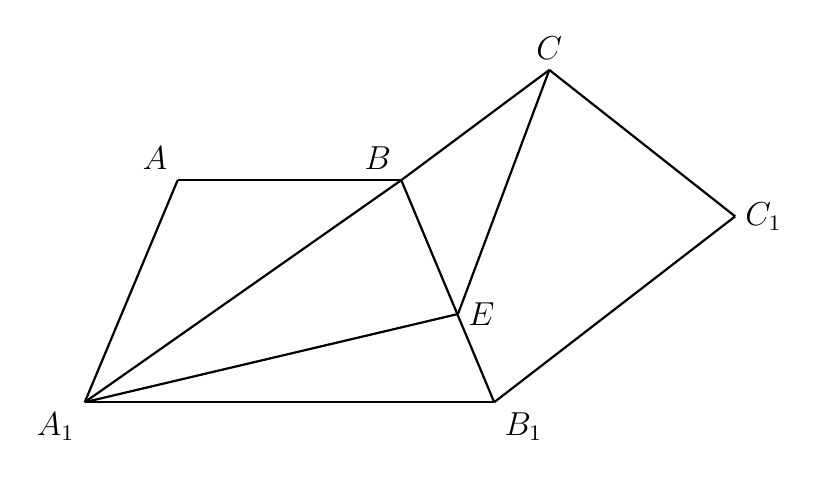
\begin{tikzpicture}[line width=0.8pt, font=\large]
  \coordinate (A) at (2.78,-2.74);
  \coordinate (B) at (5.62,-2.74);
  \coordinate (C) at (7.5,-1.34);
  \coordinate (C1) at (9.86,-3.2);
  \coordinate (B1) at (6.8,-5.56);
  \coordinate (E) at (6.34,-4.44);
  \coordinate (A1) at (1.6,-5.56);

  \draw (A1) -- (A);
  \draw (A) -- (B);
  \draw (B) -- (C);
  \draw (C) -- (C1);
  \draw (C1) -- (B1);
  \draw (B1) -- (A1);
  \draw (A1) -- (B);
  \draw (A1) -- (E);
  \draw (E) -- (C);
  \draw (B) -- (B1);

  \node[above left] at (A) {$A$};
  \node[above left] at (B) {$B$};
  \node[above] at (C) {$C$};
  \node[right] at (C1) {$C_1$};
  \node[below right] at (B1) {$B_1$};
  \node[right] at (E) {$E$};
  \node[below left] at (A1) {$A_1$};
\end{tikzpicture}
\end{document}
